% !TEX root = ../main.tex

% WebAgent: From Raw Trajectories to a Trained Small Language Model

% Shorthand commands for long module image filenames
\newcommand{\modprefix}{d__4_thesis_lab_WebAgentExperiment_docs_notebooks_module_diagram_module_}
\newcommand{\modI}{\modprefix 1_browser_agent_components.png}
\newcommand{\modII}{\modprefix 2_raw_loader_components.png}
\newcommand{\modIII}{\modprefix 3_action_extractor_components.png}
\newcommand{\modIV}{\modprefix 4_operation_normalizer_components.png}
\newcommand{\modV}{\modprefix 5_candidate_builder_components.png}
\newcommand{\modVI}{\modprefix 6_html_generator_components.png}
\newcommand{\modVII}{\modprefix 7_action_repr_builder_components.png}
\newcommand{\modVIII}{\modprefix 8_trajectory_builder_components.png}

%%% ============================================================
\section{Project Overview}
%%% ============================================================

\subsection{Objective \& Three-Phase Pipeline}
\begin{frame}{\insertsubsection}
  \textbf{Objective:} Train a Small Language Model (SLM) to autonomously navigate
  web interfaces by learning from recorded human-like agent sessions.

  \vspace{0.3cm}
  \textbf{Three-phase pipeline:}
  \begin{enumerate}
    \item \textbf{Phase 1 --- Data Processing:} Clean and convert raw browser
          interaction logs into structured training data
    \item \textbf{Phase 2 --- Model Training:} Fine-tune a pre-trained SLM using
          Supervised Fine-Tuning (SFT) with LoRA adapters
    \item \textbf{Phase 3 --- Deployment:} Package the training environment into a
          portable Docker image for cloud execution
  \end{enumerate}
\end{frame}

%%% ============================================================
\section{Part 1: Data Processing}
%%% ============================================================

\subsection{Purpose of the Data Processing Pipeline}
\begin{frame}{\insertsubsection}
  \textbf{Input:} Raw browser session logs recorded by an AI agent navigating a web store.

  \vspace{0.2cm}
  \textbf{Problem:} Raw logs are noisy, inconsistently structured, and contain bad
  sessions that would corrupt the model if used directly for training.

  \vspace{0.2cm}
  \textbf{Goal:} Transform raw logs into clean, labeled question--answer pairs that
  a language model can learn from.

  \vspace{0.2cm}
  \textbf{Pipeline at a glance:}

  \vspace{0.1cm}
  \scriptsize
  \begin{center}
    Raw logs $\;\rightarrow\;$ Format $\;\rightarrow\;$ Clean $\;\rightarrow\;$
    Validate $\;\rightarrow\;$ Flatten $\;\rightarrow\;$ Build DOM
    $\;\rightarrow\;$ Format Q\&A $\;\rightarrow\;$ Write
  \end{center}
  \normalsize
\end{frame}

\begin{frame}{Preprocessing Pipeline: All 7 Modules}
  \begin{center}
    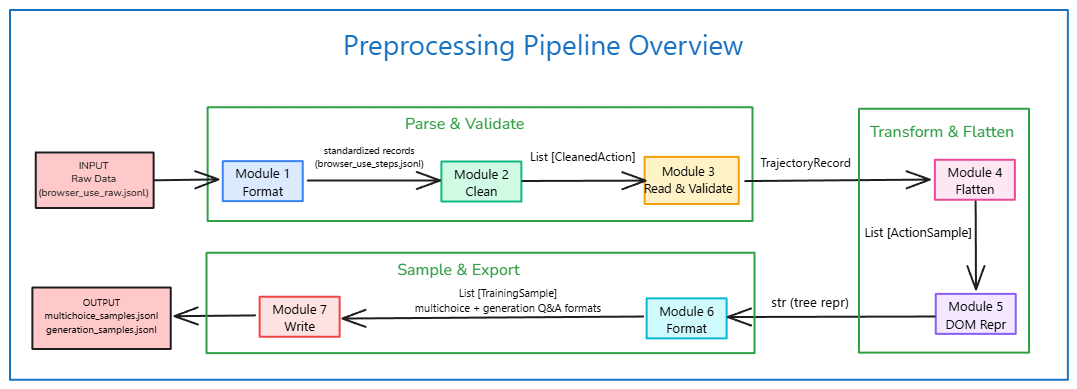
\includegraphics[width=\linewidth,height=0.72\textheight,keepaspectratio]{pipeline.png}
  \end{center}
  \vspace{0.05cm}
  {\scriptsize\textit{Seven modules grouped into three stages: \textbf{Parse \& Validate} (Phase 2, Modules 1--2), \textbf{Transform \& Flatten} (Phase 3, Modules 3--5), and \textbf{Sample \& Export} (Phase 3, Modules 6--7). Data flows left-to-right from raw browser logs to training JSONL files.}}
\end{frame}

\subsection{Phase 2: Collecting \& Cleaning Trajectories}
\begin{frame}{\insertsubsection}
  \textbf{What is a trajectory?}
  A single recorded agent session --- a sequence of actions (click, type, scroll)
  performed to complete one task on the website.

  \vspace{0.2cm}
  \textbf{Module 1 --- Format:} Converts raw JSON session dumps into a standardized
  structure, normalizing field names and action representations.

  \vspace{0.2cm}
  \textbf{Module 2 --- Clean} (four filtering passes):

  \vspace{0.1cm}
  \small
  \begin{tabular}{p{0.22\textwidth} p{0.70\textwidth}}
    \textbf{Ghost drop}   & Sessions with no captured HTML                      \\
    \textbf{Loop drop}    & Sessions repeating the same action 3+ times in a row \\
    \textbf{Tail trim}    & Trailing steps that lack HTML context                \\
    \textbf{Min length}   & Sessions too short to provide meaningful signal      \\
  \end{tabular}

  \vspace{0.2cm}
  \normalsize
  \textit{Why this matters:} A single looping or empty trajectory would teach the
  model to stall or hallucinate actions.
\end{frame}

\begin{frame}{Phase 2 Diagrams: Module 1 \& 2}
  \includegraphics[width=\linewidth,height=0.34\textheight,keepaspectratio]{\modI}

  {\scriptsize\textit{\textbf{Module 1} (\texttt{main.py}): Parses raw browser JSONL, builds trajectory rows with HTML snapshots, operations, and candidate elements per step. Outputs structured \texttt{browser\_use\_steps.jsonl}.}}

  \vspace{0.15cm}
  \includegraphics[width=\linewidth,height=0.34\textheight,keepaspectratio]{\modII}

  {\scriptsize\textit{\textbf{Module 2} (\texttt{cleaner.py}): Applies six sequential filters --- ghost drop, loop drop, tail trim, min-length, and positive-candidate flagging --- producing cleaned trajectories with quality statistics.}}
\end{frame}

\subsection{Phase 3: Converting Trajectories into Training Samples}
\begin{frame}[shrink=5]{\insertsubsection}
  \textbf{Module 3 --- Validate:} Validates each record against a strict schema;
  malformed records are skipped without halting the batch.

  \vspace{0.1cm}
  \textbf{Module 4 --- Flatten:} Splits each $N$-step trajectory into $N$ independent
  training examples (task + action history + correct next action).
  \textit{A 13-step session $\rightarrow$ 13 independent training pairs.}

  \vspace{0.1cm}
  \textbf{Module 5 --- DOM Representation:} Compresses full HTML pages
  (often 50\,000+ characters) into a compact, Lisp-like tree:
  \texttt{(a id=51 meta=menuitem beauty \& personal care)}

  \vspace{0.1cm}
  \textbf{Module 6 --- Format Training Samples:} Two output formats per example:
  \begin{itemize}
    \item \textbf{Multichoice:} Model selects the correct element from lettered options
          --- trains \textit{recognition}
    \item \textbf{Generation:} Model freely describes the correct element and action
          --- trains \textit{recall}
  \end{itemize}
\end{frame}

\begin{frame}{Phase 3 Diagrams: Module 3 \& 4}
  \includegraphics[width=\linewidth,height=0.34\textheight,keepaspectratio]{\modIII}

  {\scriptsize\textit{\textbf{Module 3} (\texttt{reader.py}): Opens the cleaned JSONL, validates each line into a \texttt{TrajectoryRecord} via Pydantic, and streams valid records while enforcing min/max action-count bounds.}}

  \vspace{0.15cm}
  \includegraphics[width=\linewidth,height=0.34\textheight,keepaspectratio]{\modIV}

  {\scriptsize\textit{\textbf{Module 4} (\texttt{flattener.py}): Walks each trajectory's action list and emits one \texttt{ActionSample} per step, attaching task and session metadata --- turning an $N$-step trajectory into $N$ independent rows.}}
\end{frame}

\begin{frame}{Phase 3 Diagrams: Module 5 \& 6}
  \includegraphics[width=\linewidth,height=0.34\textheight,keepaspectratio]{\modV}

  {\scriptsize\textit{\textbf{Module 5} (\texttt{dom\_repr.py}): Parses the raw HTML with BeautifulSoup, applies \texttt{DomReprConfig} filter rules, and builds a compact Lisp-like tree string retaining only semantically meaningful elements.}}

  \vspace{0.15cm}
  \includegraphics[width=\linewidth,height=0.34\textheight,keepaspectratio]{\modVI}

  {\scriptsize\textit{\textbf{Module 6} (\texttt{formatter.py}): Takes each \texttt{ActionSample} + DOM tree and produces two training records --- a multiple-choice sample (recognition) and a free-generation sample (recall) --- then serializes them.}}
\end{frame}

\begin{frame}{Phase 3 Diagrams: Module 7 \& 8}
  \includegraphics[width=\linewidth,height=0.34\textheight,keepaspectratio]{\modVII}

  {\scriptsize\textit{\textbf{Module 7} (\texttt{writer.py}): Receives formatted sample dicts, writes multichoice and generation records to separate JSONL files, and flushes with final \texttt{WriterStats}.}}

  \vspace{0.15cm}
  \includegraphics[width=\linewidth,height=0.34\textheight,keepaspectratio]{\modVIII}

  {\scriptsize\textit{\textbf{Module 8} (\texttt{pipeline.py}): Top-level orchestrator that chains all Phase 3 modules --- Load Config $\to$ Iter Trajectories $\to$ Flatten $\to$ Build Tree Repr $\to$ Format Samples $\to$ Write --- and returns \texttt{PipelineStats}.}}
\end{frame}

%%% ============================================================
\section{Part 2: Training the Small Language Model}
%%% ============================================================

\subsection{Training Data: Format and Split}
\begin{frame}{\insertsubsection}
  \textbf{Base model:} Qwen3.5-9B --- a 9B-parameter causal language
  model pre-trained on general text.

  \vspace{0.15cm}
  \textbf{Data source:} \texttt{generation\_samples.jsonl} (Phase 3 output)

  \vspace{0.1cm}
  \footnotesize
  \setlength{\tabcolsep}{4pt}
  \begin{tabular}{p{0.18\textwidth} p{0.16\textwidth} p{0.50\textwidth}}
    \textbf{Field}        & \textbf{Role}  & \textbf{Example}                     \\
    \hline
    \texttt{seq\_context} & Page context   & \texttt{(nav id=1)(a id=51 ...)}     \\
    \texttt{seq\_in}      & Question       & \textit{``Task: Add 3 products ...''} \\
    \texttt{seq\_out}     & Answer         & \textit{``Element: (a id=51) CLICK''} \\
  \end{tabular}
  \normalsize

  \vspace{0.15cm}
  \normalsize
  \textbf{Split:} $\sim$1,174 samples $\;\rightarrow\;$
  85\% train ($\sim$998) / 15\% validation ($\sim$176), shuffled.
\end{frame}

\subsection{Tokenization}
\begin{frame}{\insertsubsection}
  \textbf{What tokenization does:} Converts raw text (prompt + completion) into
  integer token sequences that the model can process.

  \vspace{0.1cm}
  \begin{center}
    Raw text $\;\rightarrow\;$ Tokenizer $\;\rightarrow\;$
    \texttt{input\_ids} + \texttt{attention\_mask} + \texttt{labels}
  \end{center}

  \small
  \begin{tabular}{p{0.28\textwidth} p{0.64\textwidth}}
    \textbf{Output}           & \textbf{Purpose}                                     \\
    \hline
    \texttt{input\_ids}        & Integer representation of each token                \\
    \texttt{attention\_mask}   & Marks real tokens vs.\ padding                      \\
    \texttt{labels}            & Mirrors \texttt{input\_ids}; prompt tokens masked with \texttt{-100} \\
  \end{tabular}

  \vspace{0.1cm}
  \normalsize
  \textbf{Completion-only loss:} Prompt tokens are excluded from the loss via label
  masking --- the model is penalized only for incorrect \textit{answers}.

  \vspace{0.1cm}
  \textbf{Max sequence length:} 2,048 tokens; context $>$ 6,000 characters is
  truncated before tokenization.
\end{frame}

\subsection{Model Configuration: SFT + LoRA}
\begin{frame}{\insertsubsection}
  \textbf{Approach:} Parameter-Efficient Fine-Tuning (PEFT) --- adapting a frozen
  base model by training a small set of additional weights.

  \vspace{0.1cm}
  \textbf{Why LoRA?} Instead of updating all 9B parameters, LoRA inserts small
  trainable adapter matrices. Only $\sim$1.3\% of parameters are trained.

  \vspace{0.1cm}
  \small
  \begin{tabular}{p{0.28\textwidth} p{0.11\textwidth} p{0.46\textwidth}}
    \textbf{Parameter}   & \textbf{Value} & \textbf{Effect}                     \\
    \hline
    Rank $r$             & 32             & Capacity of adapter matrices        \\
    Alpha                & 64             & Scaling factor (alpha/$r$ = 2)      \\
    Dropout              & 0.05           & Regularization during training      \\
    Target layers        & 7 layers       & Attention + feed-forward components \\
  \end{tabular}

  \vspace{0.15cm}
  \normalsize
  \textbf{QLoRA (4-bit):} Frozen base model compressed from FP16 to 4-bit,
  reducing VRAM by $\sim$4$\times$ while computing in BF16.

  \begin{center}
    \small
    FP16: $\sim$3 GB VRAM $\;\rightarrow\;$ 4-bit: $\sim$1 GB VRAM
  \end{center}
\end{frame}

\subsection{Training Configuration: Hyperparameters}
\begin{frame}{\insertsubsection}
  \footnotesize
  \setlength{\tabcolsep}{4pt}
  \begin{tabular}{p{0.34\textwidth} p{0.18\textwidth} p{0.38\textwidth}}
    \textbf{Parameter}         & \textbf{Value}    & \textbf{Rationale}             \\
    \hline
    Epochs                     & 5                 & Full passes through dataset    \\
    Batch size                 & 4 per GPU         & Memory vs.\ throughput balance \\
    Gradient accumulation      & 2 steps           & Effective batch size = 8       \\
    Learning rate              & $2\times10^{-4}$  & Standard for LoRA              \\
    LR schedule                & Cosine decay      & 10\% warmup                    \\
    Optimizer                  & Paged AdamW 8-bit & $\sim$50\% optimizer memory    \\
    Weight decay               & 0.01              & Light regularization           \\
  \end{tabular}
\end{frame}

\subsection{Training Configuration: Efficiency Techniques}
\begin{frame}{\insertsubsection}
  \textbf{Efficiency techniques:}
  \small\raggedright
  \begin{itemize}
    \item \textbf{Sample packing} --- fills each 2,048-token window completely,
          maximizing GPU utilization
    \item \textbf{Liger Kernel} --- CUDA kernels: $\sim$20\% faster,
          $\sim$60\% less activation memory
    \item \textbf{Flash Attention 2} --- $\sim$2$\times$ faster,
          $\sim$3$\times$ less memory
    \item \textbf{Gradient checkpointing} --- recomputes activations during
          backprop; trades compute for memory
  \end{itemize}
\end{frame}

\subsection{Training Pipeline \& Checkpointing}
\begin{frame}[fragile]{\insertsubsection}
  \textbf{Training loop:}
\begin{verbatim}
For each epoch (x5):
  For each packed batch:
    1. Forward pass -> predict completion tokens
    2. Compute loss on completion tokens only
    3. Backpropagate -> compute gradients
    4. Update LoRA adapter weights (base frozen)
  -> Evaluate on validation set (eval_loss)
  -> Save checkpoint
-> Restore checkpoint with lowest eval_loss
\end{verbatim}

  \textbf{Checkpointing strategy:}
  \begin{itemize}
    \item Checkpoint saved \textbf{after every epoch}; \textbf{2 most recent} kept
    \item Best checkpoint (lowest \texttt{eval\_loss}) auto-restored at end
  \end{itemize}
\end{frame}

\subsection{Output Artifact}
\begin{frame}{\insertsubsection}
  \textbf{Final output:}
  \begin{center}
    \texttt{data/checkpoints/sft\_lora/final\_adapter/}
  \end{center}

  \begin{itemize}
    \item \texttt{adapter\_config.json} --- LoRA configuration
    \item \texttt{adapter\_model.safetensors} --- trained weights (\textbf{$\sim$80 MB})
    \item Tokenizer files
  \end{itemize}

  \vspace{0.3cm}
  \textbf{Key insight:} Only the adapter is saved --- \textbf{not} the full base model.

  \begin{center}
    Adapter: $\sim$80 MB \quad vs \quad Base model: $\sim$3 GB
  \end{center}

  The base model is downloaded separately and remains reusable across experiments.
\end{frame}

%%% ============================================================
\section{Part 3: Dockerization \& Cloud Deployment}
%%% ============================================================

\subsection{Why Docker and How It Works}
\begin{frame}{\insertsubsection}
  \textbf{Problem:} The training environment requires a precise stack ---
  specific versions of PyTorch, CUDA, Flash Attention, bitsandbytes ---
  that is error-prone to set up manually on cloud machines.

  \vspace{0.15cm}
  \textbf{Solution:} Package the entire environment into a Docker image.

  \vspace{0.1cm}
  \small
  \begin{tabular}{p{0.22\textwidth} p{0.70\textwidth}}
    \textbf{Layer}    & \textbf{Content}                                              \\
    \hline
    Base              & PyTorch 2.3.1 + CUDA 12.1 + cuDNN 8 (official image)         \\
    System tools      & \texttt{build-essential}, \texttt{ninja-build} (for Flash Attn) \\
    Flash Attention   & Compiled from source for Ampere (A100) \& Ada (RTX 40xx)     \\
    ML packages       & \texttt{transformers}, \texttt{peft}, \texttt{trl}, \texttt{bitsandbytes}, etc. \\
    Training script   & \texttt{scripts/train\_sft\_lora.py}                          \\
  \end{tabular}

  \vspace{0.15cm}
  \normalsize
  \textbf{Key design:} Training data and checkpoints are \textbf{not} baked into
  the image --- they are mounted as volumes at runtime, keeping the image generic
  and reusable.
\end{frame}

\subsection{Cloud Deployment Workflow}
\begin{frame}[fragile,shrink=10]{\insertsubsection}
  \textbf{Target:} Any cloud GPU provider (Vast.ai, RunPod, Lambda Labs)
  with an Ampere or newer GPU.

\begin{verbatim}
1. Build:   docker build -f docker/train.Dockerfile \
                         -t webagent-train .
2. Test:    docker compose run train --smoke-test
3. Push:    docker push <user>/webagent-train:latest
4. Rent GPU on Vast.ai; set HF_TOKEN env var
5. Upload:  scp data/training/... user@host:/workspace/
6. Train:   python scripts/train_sft_lora.py --bf16
7. Fetch:   scp -r user@host:.../checkpoints ./
\end{verbatim}

  \small
  \begin{tabular}{p{0.22\textwidth} p{0.14\textwidth} p{0.24\textwidth} p{0.20\textwidth}}
    \textbf{GPU}     & \textbf{VRAM} & \textbf{Train time} & \textbf{Cost}   \\
    \hline
    RTX 4090         & 24 GB         & $\sim$25 min        & \$0.45/hr       \\
    A100 (40 GB)     & 40 GB         & $\sim$10 min        & \$1.50/hr       \\
  \end{tabular}
\end{frame}

%%% ============================================================
\section{Summary}
%%% ============================================================

\subsection{End-to-End Pipeline}
\begin{frame}[fragile]{\insertsubsection}
\begin{verbatim}
Browser session logs
      |  Format . Clean . Validate       (Phase 2)
Cleaned trajectories
      |  Flatten . DOM Repr . Format Q&A (Phase 3)
generation_samples.jsonl  (~1,174 pairs)
      |  Tokenize . Pack . SFT + LoRA   (Training)
final_adapter/  (~80 MB LoRA on Qwen2.5-1.5B)
      |  Docker image
Deployable training environment (any cloud GPU)
\end{verbatim}
\end{frame}

\subsection{Key Design Decisions}
\begin{frame}{\insertsubsection}
  \small
  \begin{tabular}{p{0.40\textwidth} p{0.52\textwidth}}
    \textbf{Decision}              & \textbf{Rationale}                                    \\
    \hline
    LoRA over full fine-tuning     & Trains only 1.3\% of parameters --- fits one consumer GPU \\
    QLoRA 4-bit quantization       & 4$\times$ VRAM reduction with minimal accuracy loss   \\
    Completion-only loss           & Model learns actions, not to re-read page content     \\
    DFT loss term                  & Prevents catastrophic forgetting of general language  \\
    Docker packaging               & One-command reproducible env on any cloud provider    \\
    Adapter-only artifact          & 80 MB deliverable; base model unchanged \& reusable   \\
  \end{tabular}
\end{frame}
